\documentclass[11pt]{article}

\usepackage[preprint]{acl}

\usepackage{times}
\usepackage{latexsym}
\usepackage[T1]{fontenc}
\usepackage[utf8]{inputenc}
\usepackage{amsmath}
\usepackage{microtype}
\usepackage{inconsolata}
\usepackage{graphicx}
\usepackage{booktabs}
\usepackage{enumitem}
\usepackage{pgfplots}
\usepackage{tikz}
\pgfplotsset{compat=1.16}
\definecolor{seriesA}{HTML}{2A78D6}
\definecolor{seriesB}{HTML}{EB6834}
\definecolor{seriesC}{HTML}{1BAF7A}

\title{Reasoning, Not Debate, Repairs Encoding-Fragile Graph Reasoning in LLMs}

\author{Itai Paperno \\
  \texttt{itaipaperno@mail.tau.ac.il} \\\And
  Roi Guri \\
  \texttt{roiguri@mail.tau.ac.il} \\\And
  Shahar Cohen \\
  \texttt{shaharc6@mail.tau.ac.il} \\}

\begin{document}
\maketitle

\begin{abstract}
Large language models answer the same graph question with sharply different
accuracy depending only on how the graph is serialized into text - a robustness
gap we confirm on Llama-3.3-70B. A natural remedy is multi-agent
debate: a Critic checks a Proposer's reasoning before it is committed.
Debate rests on a verification asymmetry - checking a claim should be
cheaper than producing one - and graph reasoning is an unusually clean place to
test it, because an edge claim is objectively present in the serialization or it
is not. Across three tasks, three encodings, and three seeds, we find that debate
does raise accuracy and does narrow the encoding gap. However, decomposing the
debate into its reasoning scaffold and its verify-and-revise loop shows that the
entire gain comes from asking the model to reason: the loop itself contributes
nothing. A compute-matched majority vote over independent reasoned answers beats
debate on every cell at comparable token cost. Encoding fragility is real and
reasoning reduces it - but the multi-agent structure is not why.
\end{abstract}

\section{Introduction}

Large language models (LLMs) are increasingly asked to reason over graph-structured
data - social networks, knowledge graphs, dependency structures - presented as
text. A recurring and uncomfortable finding is that their accuracy is highly
sensitive to how the graph is written down: the same graph and the same
question, serialized under a different but equally faithful convention, can move
accuracy by tens of points \citep{fatemi2024talk}. We reproduce this
encoding fragility on Llama-3.3-70B: a
\texttt{connected\_nodes} query answered correctly $95.8\%$ of the time under one
serialization drops to $48.8\%$ under another, on the same graphs. A strong dependence on notation indicates that the phrasing of the input, not the
graph's structure, is driving the model's answers.

A natural remedy is multi-agent debate: a Proposer produces an answer and a
Critic scrutinizes it before it is committed, a procedure reported to improve
factuality and reasoning \citep{du2023debate}. Debate rests on an implicit
verification asymmetry: recognizing that a claim is wrong is assumed to be
cheaper than producing the right claim in the first place \citep{irving2018debate}.
Yet the evidence is mixed - when debate is placed head-to-head against simple
aggregation it does not always win \citep{choi2025debateorvote}. These results are hard to
interpret because in most reasoning domains the steps a Critic checks are not
objectively verifiable.

Graph reasoning removes that obstacle. An atomic claim in a Proposer's
trace - ``node $5$ is adjacent to node $13$'' - either appears in the serialized
graph or it does not, so a Critic's job is objectively unambiguous and its behavior
can be measured exactly. This makes graphs an ideal setting for the question we
ask: does debate reduce encoding fragility, and if it helps at all, is the
multi-agent structure the reason?

We run three graph tasks (\texttt{edge\_existence}, \texttt{node\_degree},
\texttt{connected\_nodes}) under three encodings (\texttt{adjacency},
\texttt{incident}, \texttt{friendship}) across three independent seeds, comparing a
zero-shot baseline, a Proposer--Critic debate, and a compute-matched majority vote.
Our findings are:

\begin{itemize}[nosep]
  \item \textbf{Encoding fragility is large and significant} on all three tasks,
    unanimously worst under \texttt{friendship} and best under \texttt{incident}
    (\S\ref{sec:results}).
  \item \textbf{Debate raises accuracy and narrows the encoding gap.}
  \item \textbf{The gain is the reasoning, not the debate.} Decomposing
    debate into its first-turn chain-of-thought and its verify-and-revise loop,
    the loop contributes nothing: asking the model to reason helps, having a Critic
    argue about the reasoning does not.
  \item \textbf{A compute-matched majority vote beats debate} on every cell at
    $1.07\times$ its token cost. The Critic detects real errors, but acting on
    its verdicts hurts more than it helps.
\end{itemize}

\noindent The takeaway is a positive result wrapped around a negative one: encoding
fragility is real and reasoning genuinely reduces it, but the multi-agent debate
structure - the part that is expensive and elaborate - is not what does the work.

\section{Related Work}
\label{sec:related}

\paragraph{LLM reasoning over serialized graphs.}
A body of recent work studies how well LLMs answer questions about graphs given as
text, and consistently finds that the choice of encoding - how nodes,
edges, and structure are rendered into a string - is a primary factor in
accuracy. \citet{fatemi2024talk} systematically vary graph encodings and show that
model performance swings widely across them, with no single encoding dominant
across tasks. Building on that work, \citet{perozzi2024graphtoken} learn a
structured encoding fed directly to the LLM - an alternative to our method, which
leaves the text input unchanged and instead has the model reason more at inference
time. We take this fragility as our starting point, measuring the accuracy gap
across encodings and asking whether reasoning can shrink it. % ADD: a GraphQA / LLM-graph-reasoning survey or benchmark citation

\paragraph{Multi-agent debate.}
Debate frames inference as an interaction between models that argue toward a
better answer. \citet{irving2018debate} introduce debate as a scalable-oversight
mechanism: two agents argue over a question and a weaker judge rules between them,
the hope being that a limited judge can supervise stronger agents because exposing
a flaw is easier than committing one. \citet{du2023debate} realize this empirically
for LLMs, having several instances propose answers and critique one another over
multiple rounds until they converge, which improves factuality, commonsense, and
arithmetic reasoning. The mechanism rests entirely on this verification asymmetry,
and the assumption is not guaranteed: \citet{barnes2020obfuscated} identify an
obfuscated-arguments problem, in which a debater constructs an argument whose flaw
neither side can efficiently locate, so refuting a wrong claim is no cheaper than
producing a right one. Our Proposer--Critic setup is a deliberately minimal,
two-role instance of this family: a single model produces one answer, then
critiques and revises it. We expect graphs to avoid the obfuscated-arguments
problem, since every claim is verifiable and any flaw can be caught.

\paragraph{Aggregation as the alternative.}
A simpler way to spend extra inference compute is to sample several answers
independently and aggregate them. Chain-of-thought prompting \citep{wei2022cot}
has the model produce intermediate reasoning steps before its answer, improving
accuracy on multi-step problems; this is the same reasoning we isolate as debate's
first turn. Self-consistency \citep{wang2023selfconsistency} samples several such
reasoning paths independently and returns the majority answer, reliably improving
accuracy - which is exactly our majority-vote arm. This makes voting the natural
control for debate: both spend more compute than a single answer, but debate lets
the attempts interact while voting keeps them independent.
\citet{choi2025debateorvote} compare the two and find voting competitive with or
better than debate in several settings. We sharpen this comparison in two ways:
we match compute between the two arms by measured token cost rather than response
count, and we run it where debate should do best - a fragile, checkable task with
real errors for the Critic to catch.

% ============================================================
% TODO sections below  -  stubbed so the document compiles.
% ============================================================

\section{Setup}
\label{sec:setup}

\paragraph{Data.}
We generate undirected Erd\H{o}s--R\'enyi graphs with NetworkX
\citep{hagberg2008networkx}, $5$ to $19$ nodes each and edge probability drawn per
graph, giving a wide spread of densities. For each of three seeds
($7$, $11$, $13$) we draw an independent set of $200$ graphs, and every graph is
rendered under all three encodings, so a per-encoding accuracy difference reflects
the encoding alone and all comparisons across encodings are paired by graph.

\paragraph{Tasks and encodings.}
We study three tasks, spanning boolean, integer, and set answers, and three
encodings from \citet{fatemi2024talk}; Table~\ref{tab:example} defines each with an
example. The encodings preserve the graph exactly and differ only in surface form,
labeling nodes with integers except \texttt{friendship}, which uses popular names.
Crossing $3$ tasks $\times$ $3$ encodings $\times$ $3$ seeds $\times$ $200$ graphs
gives $9$ cells of $n=600$ each, $5{,}400$ instances per condition.

\begin{table}[t]
  \centering
  \small
  \begin{tabular}{@{}p{0.29\columnwidth}p{0.63\columnwidth}@{}}
    \toprule
    \multicolumn{2}{@{}c@{}}{\textbf{Graph}}\\
    \addlinespace
    \multicolumn{2}{@{}c@{}}{%
      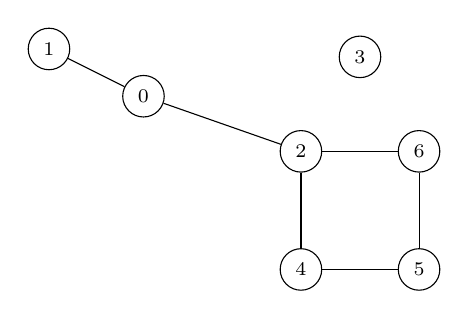
\begin{tikzpicture}[baseline,
          every node/.style={circle,draw,fill=white,inner sep=0pt,
            minimum size=15pt,font=\scriptsize}]
        \node (n0) at (-2.0,0.7)  {0};
        \node (n1) at (-3.2,1.3)  {1};
        \node (n2) at (0,0)       {2};
        \node (n6) at (1.5,0)     {6};
        \node (n4) at (0,-1.5)    {4};
        \node (n5) at (1.5,-1.5)  {5};
        \node (n3) at (0.75,1.2)  {3};
        \draw (n0)--(n1); \draw (n0)--(n2);
        \draw (n2)--(n4); \draw (n2)--(n6);
        \draw (n4)--(n5); \draw (n5)--(n6);
      \end{tikzpicture}}\\
    \midrule
    \multicolumn{2}{@{}c@{}}{\textbf{Encodings}}\\
    \addlinespace
    \texttt{adjacency} & The edges in G are: (0, 1) (0, 2) (2, 4)
      (2, 6) (4, 5) (5, 6). \\
    \addlinespace
    \texttt{incident} & Node 0 is connected to nodes
      1, 2. Node 2 to 0, 4, 6. Node 4 to 2, 5. Node 5 to 4, 6. Node 6 to 2, 5. \\
    \addlinespace
    \texttt{friendship} & James and Robert are
      friends. James and John are friends. John and David are friends. John and
      Patricia are friends. David and Mary are friends. Mary and Patricia are
      friends. \\
    \midrule
    \multicolumn{2}{@{}c@{}}{\textbf{Tasks}}\\
    \addlinespace
    \texttt{edge\_existence} & Is node 6 connected to node 1? \newline No. \\
    \addlinespace
    \texttt{node\_degree} & What is the degree of node 5? \newline 2. \\
    \addlinespace
    \texttt{connected\_nodes} & List all nodes connected to 2. \newline
      0, 4, 6. \\
    \bottomrule
  \end{tabular}
  \caption{One graph under the three encodings and the three tasks. All encodings
  are information-preserving re-serializations of the same graph.}
  \label{tab:example}
\end{table}

\paragraph{Model and conditions.}
All conditions use \texttt{Llama-3.3-70B-Instruct-Turbo} (FP8). We compare three
conditions. The baseline is a
single zero-shot answer-only response. Debate is a Proposer--Critic loop:
the Proposer emits a numbered claim trace and a final answer, the Critic reviews it
against the encoding and returns \textsc{agree} or \textsc{revise}, and the Proposer
revises until agreement or a turn budget is reached; the Proposer and Critic are the
same model in different roles. Its first turn is a single-turn
chain-of-thought answer under the same decoding, which lets us separate the
reasoning (baseline\,$\rightarrow$\,turn~1) from the
verify-and-revise loop (turn~1\,$\rightarrow$\,final) with no extra runs.
Majority vote draws the same Proposer prompt $N{=}3$ times independently at
the model's shipped sampling defaults and returns the majority answer across the
three; it differs from debate in exactly one thing - whether the attempts see each
other.

\paragraph{Matched compute.}
$N{=}3$ was fixed before the run by matching debate's measured token spend
(debate buys $2.6$--$2.9$ turn-1-equivalents per instance). The realized cost is
$1{,}664$ tokens per instance for the vote against $1{,}554$ for debate, so the two
arms are compute-matched to within $7\%$ and any advantage the vote shows is not an
artifact of the budget. The sampling temperature is Llama's shipped
default, fixed before any result; we report how often the three samples disagreed as
a diagnostic, but never tuned the temperature to change it.

\paragraph{Metrics and statistics.}
The primary metric is accuracy; the secondary is encoding fragility, the
cross-encoding accuracy spread (max\,$-$\,min) within a task. Because encodings are
paired by graph, significance uses paired tests: Cochran's $Q$ as an overall test across
a task's three encodings, and McNemar's test for pairwise gaps and for
condition-vs-condition accuracy differences; cell accuracies carry Wilson intervals.
The Critic diagnostic (does a \textsc{revise} track the answer actually being
wrong?) is unpaired, one observation per verdict, so it takes a $\chi^2$ association
test reported with the signed $\phi$. We report the fragility spread descriptively,
supported by replication across the three independent seeds rather than by a test of
the spread itself. Finally, \texttt{edge\_existence} is a single-pair lookup whose
trace reduces to one atomic claim, so a claim-by-claim critique has nothing to work
on and its baseline sits near ceiling; it behaves as a control rather than a
third fragile task, and we report every result both over all $9$ cells and over the
$6$ cells that exclude it.

\section{Results and Analysis}
\label{sec:results}

\subsection{Encoding fragility is large}
\label{sec:frag}
Baseline accuracy swings sharply with the serialization on all three tasks
(Table~\ref{tab:fragility}), reaching a $0.470$ gap on \texttt{connected\_nodes}
between the same graphs. The effect is highly significant on every task under the
paired Cochran's $Q$ test (all $p<0.001$), and its shape is unanimous:
\texttt{incident} is the best encoding and \texttt{friendship}, the one encoding
that names nodes rather than numbering them, the worst on all three. This fragility
is the phenomenon the rest of the paper asks a reasoning procedure to repair.

\begin{table*}[t]
  \centering
  \small
  \begin{tabular}{@{}lccccc@{}}
    \toprule
    \textbf{Task} & \texttt{incident} & \texttt{adjacency} & \texttt{friendship} &
      \textbf{Spread (max$-$min)} & \textbf{Cochran $Q$} \\
    \midrule
    \texttt{connected\_nodes} & 0.958 & 0.743 & 0.488 & 0.470 & 377 \\
    \texttt{node\_degree}     & 0.873 & 0.655 & 0.637 & 0.237 & 148 \\
    \texttt{edge\_existence}  & 0.980 & 0.938 & 0.867 & 0.113 &  81 \\
    \bottomrule
  \end{tabular}
  \caption{Baseline accuracy per encoding, with the cross-encoding spread and
  Cochran's $Q$. \texttt{edge\_existence} is the near-ceiling control.}
  \label{tab:fragility}
\end{table*}

\begin{figure}[t]
  \centering
  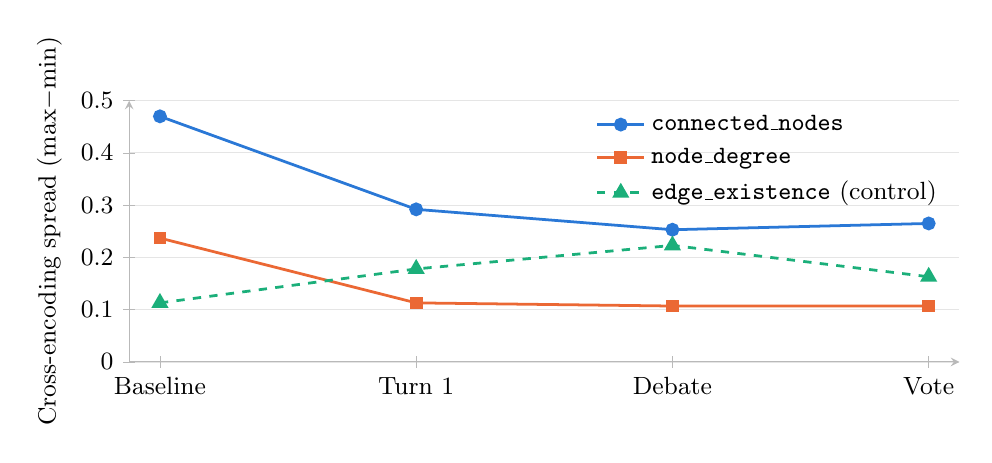
\begin{tikzpicture}
    \begin{axis}[
      width=\columnwidth,
      height=4.9cm,
      xtick={0,1,2,3},
      xticklabels={Baseline,{Turn 1},Debate,Vote},
      xmin=-0.12, xmax=3.12,
      ymin=0, ymax=0.5,
      ytick={0,0.1,0.2,0.3,0.4,0.5},
      ylabel={Cross-encoding spread (max$-$min)},
      ylabel style={font=\small},
      tick label style={font=\small},
      ymajorgrids=true,
      grid style={gray!20, line width=0.3pt},
      axis lines=left,
      axis line style={gray!55},
      tick style={gray!55},
      legend style={draw=none, fill=none, font=\small, at={(0.99,0.99)},
        anchor=north east, cells={anchor=west}, row sep=1pt},
      mark options={solid},
    ]
    \addplot[seriesA, line width=1pt, mark=*, mark size=2pt]
      coordinates {(0,0.470)(1,0.292)(2,0.253)(3,0.265)};
    \addlegendentry{\texttt{connected\_nodes}}
    \addplot[seriesB, line width=1pt, mark=square*, mark size=1.8pt]
      coordinates {(0,0.237)(1,0.113)(2,0.107)(3,0.107)};
    \addlegendentry{\texttt{node\_degree}}
    \addplot[seriesC, line width=1pt, dashed, mark=triangle*, mark size=2.6pt]
      coordinates {(0,0.113)(1,0.178)(2,0.223)(3,0.163)};
    \addlegendentry{\texttt{edge\_existence} (control)}
    \end{axis}
  \end{tikzpicture}
  \caption{Cross-encoding accuracy spread (max$-$min) by stage for each task; lower
  is less fragile.}
  \label{fig:fragility}
\end{figure}

\subsection{Debate raises accuracy and narrows the gap}
\label{sec:apparent}
Debate raises mean accuracy over the baseline by $+0.050$ over all nine cells
(McNemar $b/c=351/619$, $p<0.001$; Table~\ref{tab:main}), replicating in
sign across all three independent seeds. It also narrows the encoding gap
(Figure~\ref{fig:fragility}): the \texttt{connected\_nodes} spread falls
$0.470\rightarrow0.253$ and \texttt{node\_degree} $0.237\rightarrow0.107$, reproducing
$3/3$ on both fragile tasks. The gains concentrate exactly where accuracy was
worst - the three largest per-cell gains are the three lowest baseline cells - so
debate works by lifting the floor, which is what narrows the spread.

\subsection{The gain is the reasoning, not the loop}
\label{sec:decomp}
Debate's first turn is a single-turn chain-of-thought answer under identical
decoding, so the split baseline\,$\rightarrow$\,turn~1\,$\rightarrow$\,final
separates the reasoning from the verify-and-revise loop
(Table~\ref{tab:main}). The reasoning accounts for the entire improvement, worth
$+0.071$ over the baseline, while the loop then reduces accuracy by $0.021$. That
damage falls on the \texttt{edge\_existence} control, where the Critic drags accuracy
from $0.922$ to $0.803$. That task has a single atomic claim: there is nothing to critique, so the
Critic only talks a correct answer down. The main takeaway is that asking
the model to reason helps; having a Critic argue about the reasoning does not.

\begin{table}[h!]
  \centering
  \small
  \begin{tabular}{@{}lcc@{}}
    \toprule
    \textbf{Condition} & \textbf{With control} & \textbf{Without control} \\
    \midrule
    Baseline                & 0.793 & 0.726 \\
    Turn 1 (CoT)            & 0.864 & 0.846 \\
    Debate (final)          & 0.843 & 0.843 \\
    Majority vote ($N{=}3$)  & \textbf{0.875} & \textbf{0.853} \\
    \midrule
    Reasoning (base$\to$T1) & $+0.071$ & $+0.120$ \\
    Loop (T1$\to$final)     & $-0.021$ & $-0.003$ \\
    Vote $-$ debate         & $+0.032$ & $+0.010$ \\
    \bottomrule
  \end{tabular}
  \caption{Mean accuracy by condition, with and without the \texttt{edge\_existence}
  control. The lower block reports the reasoning, loop, and vote$-$debate
  differences.}
  \label{tab:main}
\end{table}

Excluding the \texttt{edge\_existence} control leaves every conclusion intact
(Table~\ref{tab:main}): without the near-ceiling control, the reasoning gain grows to
$+0.120$, the loop is close to neutral ($-0.003$), and the compute-matched vote
(\S\ref{sec:vote}) still beats debate ($+0.010$).

\subsection{A compute-matched vote beats debate}
\label{sec:vote}
If the loop is not paying for its compute, the natural comparison is against
spending that compute on independent attempts instead. Majority vote scores
$0.875$ over nine cells against debate's $0.843$ ($+0.032$; $p<0.001$), at
matched compute, and it loses no cell - it is at least as
accurate as debate in all nine and better in three. The full
ordering across the arm is baseline $0.793 <$ debate $0.843 <$ turn~1 $0.864 <$ vote
$0.875$, so debate is the worst of the three reasoning conditions and is
beaten even by its own single first turn. The vote's advantage is largest on
\texttt{edge\_existence}, exactly where debate is
destructive. Because debate and the vote differ in only one thing - whether the
extra attempts interact - this isolates interaction as the ingredient that is
not paying off.

\subsection{Why the loop fails: precision, not detection}
\label{sec:mechanism}
The loop's failure is not that the Critic cannot tell right from wrong. Cross-tabbing
every verdict against whether the judged answer was actually correct, a
\textsc{revise} is strongly associated with a wrong answer (Table~\ref{tab:critic}),
and this discrimination is strongest ($\phi=+0.69$) precisely on
\texttt{edge\_existence}, where the check is a single lookup. The problem is what
detection costs: because correct answers outnumber wrong ones roughly five to one,
the Critic's false alarms on correct answers convert into more damage than its
detections repair, and revisions are net-positive in only one cell of nine. The loop
fails on \textbf{precision}, not detection - the Critic knows the answer is wrong on
\texttt{edge\_existence} and still, by revising too many correct answers, makes that
task worse.

\begin{table}[t]
  \centering
  \small
  \begin{tabular}{@{}lc@{}}
    \toprule
    \textbf{Critic diagnostic} (pooled, $5{,}825$ verdicts) & \\
    \midrule
    Base rate of wrong answers          & $0.181$ \\
    Detection rate (recall)             & $0.502$ \\
    False-alarm rate on correct answers & $0.132$ \\
    $P(\text{wrong}\mid\textsc{revise})$ & $0.459$ \\
    Association $\phi$                   & $+0.358$ \\
    Net answers flipped right\,$\to$\,wrong & $+113$ \\
    \bottomrule
  \end{tabular}
  \caption{The Critic detects half of wrong answers and a \textsc{revise} is strongly
  associated with a wrong answer ($\phi=+0.358$), but its false alarms on the far
  more numerous correct answers dominate: revisions flip $113$ more answers from right
  to wrong than the reverse. The failure is one of precision, not detection.}
  \label{tab:critic}
\end{table}

\section{Discussion}
\label{sec:discussion}

\paragraph{Reasoning repairs fragility; structure does not.}
The encoding gap does shrink under debate, but the decomposition locates the cause:
the single-turn reasoning scaffold produces essentially all of the narrowing, and a
compute-matched vote reproduces it (Table~\ref{tab:main}). What reduces a model's
sensitivity to how a graph is written down is being asked to reason about it, not the
multi-agent apparatus around that reasoning. We report the spread reduction
descriptively - it replicates across all three seeds, but we do not test the spread
itself - so the claim is that reasoning narrows the gap, not that debate confers
encoding-invariance: fragility stays highly significant under every condition.

\paragraph{The asymmetry can hold and debate still lose.}
Debate's premise - that recognizing a wrong claim is cheaper than producing a right
one - was satisfied here: the Critic discriminates right from wrong ($\phi=+0.36$,
and $+0.69$ where the check is a single lookup). Yet the loop still lost accuracy,
for a reason that is general. A verify-and-revise step changes accuracy by its
detection rate times the fraction of answers that are wrong, minus its false-alarm
rate times the fraction that are right. When a model is already mostly correct - as
Llama-3.3-70B is here, roughly five right for every one wrong - this balance tips
negative unless the Critic's precision is very high, however well it detects.
Objective checkability, the ingredient prior self-correction studies lacked, was not
enough: it sharpened detection, which was never the bottleneck, and left precision
untouched. The lesson transfers beyond graphs: self-verification pays off only where
errors are common or the check is near-perfectly precise, and neither holds for a
strong model on a task it mostly solves.

\paragraph{Spend compute on independence, not interaction.}
Because debate and the vote differ only in whether the extra attempts interact, the
comparison is a clean test of the two ways to spend inference compute, and
independence wins: three independent draws cannot argue each other out of a correct
answer, whereas a Critic can. Given a fixed budget and a task the model already
handles reasonably, sampling and voting is the safer use of it than a self-critique
loop. This does not refute debate in general - it may still help where the base error
rate is high, or where an external, reliable verifier replaces the model's own
Critic - but on encoding-fragile graph reasoning, at matched cost, it is dominated.

\section{Limitations and future work}
\label{sec:future}
\begin{itemize}[nosep,leftmargin=*]
  \item \textbf{Single model and graph regime.} Our results come from one model
    (Llama-3.3-70B) on small Erd\H{o}s--R\'enyi graphs. The net-effect account of
    \S\ref{sec:discussion} predicts the loop's sign depends on the base error rate,
    so harder tasks and weaker models are the test of whether the failure
    generalizes.
  \item \textbf{Single prompt.} We use one Proposer/Critic wording, and the Critic's
    precision may depend heavily on it; varying the prompts would separate a property
    of the method from one of the formulation.
  \item \textbf{Debate structure.} We tested one minimal two-role loop; richer
    structures - more agents, independent proposers that then interact, or multiple
    rounds - may recover value over voting.
\end{itemize}

\section{Conclusion}
\label{sec:conclusion}
LLM graph reasoning is sharply encoding-fragile, and asking the model to reason
reduces that fragility. A Proposer--Critic debate appears to help, but the gain is
entirely the reasoning it elicits: the verify-and-revise loop is inert-to-harmful,
and a compute-matched majority vote beats debate on every cell. The Critic genuinely
detects errors; it loses because, against a mostly-correct model, its false alarms
cost more than its detections repair. On this task, reasoning helps - and debate is
not why.

\bibliography{custom}

\clearpage
\appendix

\section{Prompts}
\label{sec:prompts}
Every prompt is sent as a single user message with no system prompt; the model's
chat template supplies the wrapper tokens. The question block -- the encoded graph
followed by \texttt{Q:\ \ldots} and a trailing \texttt{A:} -- is GraphQA's
\citep{fatemi2024talk} verbatim (examples in Table~\ref{tab:example}); we show the
instruction scaffolding wrapped around it, with \texttt{\{slots\}} for the
question, the running transcript, and per-task text.

\paragraph{Baseline.}
The task instruction, then the question:

{\footnotesize
\begin{verbatim}
{task instruction}

{question}
\end{verbatim}}

\noindent where \texttt{\{task instruction\}} is one of:

{\footnotesize
\begin{verbatim}
edge_existence:   Answer with exactly "Yes" or "No"
                  and nothing else.
node_degree:      Answer with a single integer (the
                  degree) and nothing else.
connected_nodes:  Answer with the connected nodes as a
                  comma-separated list (or "none" if
                  there are none) and nothing else.
\end{verbatim}}

\paragraph{Proposer (turn 1).}
Also used for each of the three majority-vote draws.

{\footnotesize
\begin{verbatim}
Answer the question below using the graph. Build the
answer as a numbered list of concise, atomic claims
-- each stating exactly one simple, verifiable fact
about the graph's nodes or edges -- then give the
final answer.
Number your claims 1., 2., 3., and so on, one claim
per line. Then write a final line that begins with
ANSWER: followed by {answer}. Write nothing after
that line.

{question}
\end{verbatim}}

\noindent \texttt{\{answer\}} is \texttt{Yes or No} (edge\_existence), \texttt{a
single integer, the degree} (node\_degree), or \texttt{the connected nodes,
comma-separated, written exactly as the graph writes them, or none}
(connected\_nodes).

\paragraph{Critic.}
The transcript is the question, the Proposer's turn-1 answer, and any later turns.

{\footnotesize
\begin{verbatim}
Another model is answering the graph question below
by writing numbered atomic claims (each about one
edge or node) and a final answer. You are the
checker; the debate so far is shown.

{transcript}

{critic cue}
\end{verbatim}}

\noindent For \texttt{node\_degree} and \texttt{connected\_nodes} the
\texttt{\{critic cue\}} is:

{\footnotesize
\begin{verbatim}
Work only from the graph text. Review the Proposer's
claims and final answer, in both directions:
- did the Proposer MISS an edge that is in the graph?
- did the Proposer INCLUDE an edge not in the graph?
AGREE only if the Proposer's supporting edges are
exactly the ones in the graph and the answer follows.
Otherwise REVISE and name each wrong edge, quoting it
from the graph's edge list. Every problem you raise
must cite an edge that actually appears in the list;
do not repeat a problem the Proposer has already
fixed. Respond in exactly this format and nothing
else:
VERDICT: AGREE
or
VERDICT: REVISE
- <an edge the Proposer missed or wrongly included,
  quoted from the graph's edge list>
\end{verbatim}}

\noindent For \texttt{edge\_existence} it is:

{\footnotesize
\begin{verbatim}
Work only from the graph text. Look in the graph's
edge list for the exact pair the question asks about,
in either order. If that pair appears, the answer is
Yes; if it does not, the answer is No -- decide this
yourself from the list. Then check the Proposer's
answer.
AGREE if the Proposer's Yes/No matches the edge list.
Otherwise REVISE and ground it: quote the queried
edge from the list if it is there, or state that no
such edge appears. Every problem you raise must be
grounded in the edge list; never invent an edge.
Respond in exactly this format and nothing else:
VERDICT: AGREE
or
VERDICT: REVISE
- <the queried edge quoted from the list, or a note
  that it does not appear>
\end{verbatim}}

\paragraph{Revision.}
The Proposer's corrected answer, given the Critic's verdict.

{\footnotesize
\begin{verbatim}
You are the Proposer in the debate below. A checker
verified your latest claims against the graph and
found problems. Produce a corrected answer that fixes
them, using the whole exchange.

{transcript}

Give your corrected answer.
Number your claims 1., 2., 3., and so on, one claim
per line. Then write a final line that begins with
ANSWER: followed by {answer}. Write nothing after
that line.
\end{verbatim}}

\end{document}
